\section{Data}
% Enumeration changed
\renewcommand{\theenumi}{/D\arabic{enumi}0/}
\renewcommand{\labelenumi}{\theenumi}

\subsection{Static data}

\begin{enumerate}
  \item Language files
  \item Manual
  \item Source Code
  \item Documentation
  \item Graphics for GUI
  \item HTML backbone
  \item Javascript files
  \item Stylesheet files
\end{enumerate}



\newpage
\subsection{Data-Warehouse data} \label{WHschema}


The data warehouse stores all the data, coming from from the databases (Skyserver) server logs.
They were subject of the ETL-process in the parser. If optional criteria are fulfilled
 they can be replaced by clearing the data warehouse 
 and loading new data via web page as administrator.

The data warehouse may use a star schema.
\begin{center}
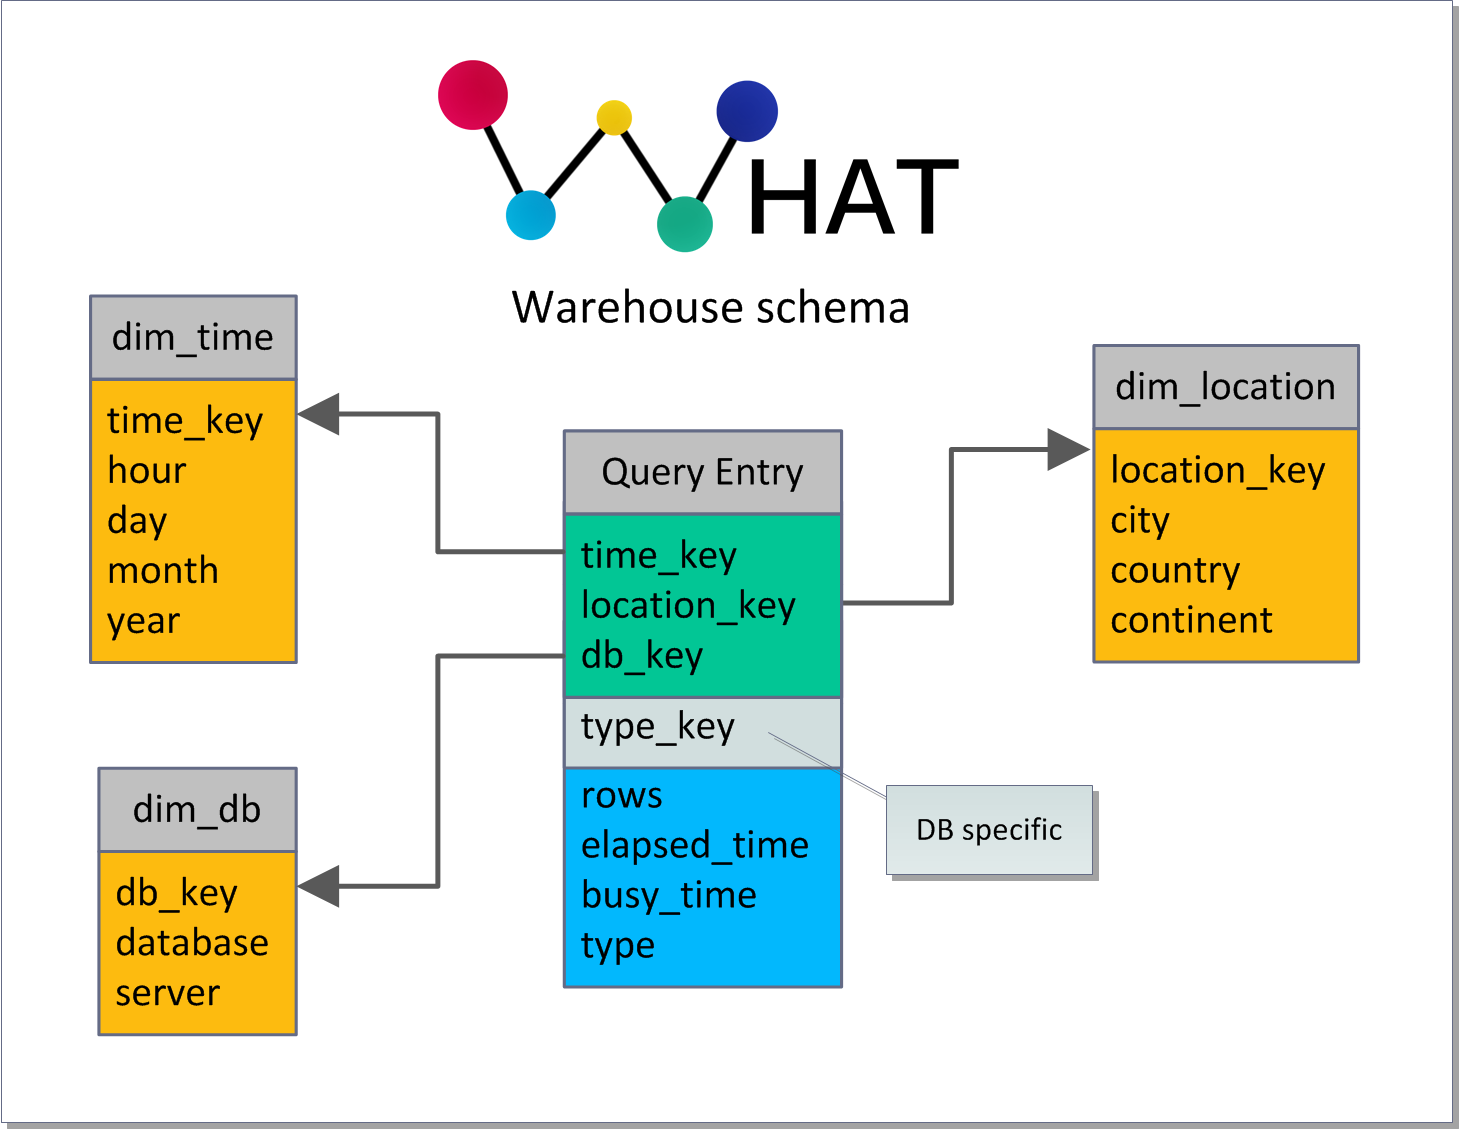
\includegraphics[width=1\linewidth]{Pictures/WareHouseSchema.png} 
\end{center}   
The column 'type\_key' can either be just a measure or refer to a new dimension. This depends on the database
on which is operated.  

See rows, elapsed time and busy time in the glossary (\ref{glos}) for descriptions. 


% \begin{enumerate}[resume] % <- resume goes on with old counter
%   \item Database accessed by Users
%   \item Server accessed by Users
%   \item City of Users
%   \item Country of Users
%   \item Time of SkyServer access
%   \item Number of rows accessed
%   \item Elapsed time of access
%   \item CPU busy time of access
% \end{enumerate}

% we may include just the schema in here? 